% Options for packages loaded elsewhere
\PassOptionsToPackage{unicode}{hyperref}
\PassOptionsToPackage{hyphens}{url}
\PassOptionsToPackage{dvipsnames,svgnames,x11names}{xcolor}
%
\documentclass[
  letterpaper,
  DIV=11,
  numbers=noendperiod]{scrartcl}

\usepackage{amsmath,amssymb}
\usepackage{iftex}
\ifPDFTeX
  \usepackage[T1]{fontenc}
  \usepackage[utf8]{inputenc}
  \usepackage{textcomp} % provide euro and other symbols
\else % if luatex or xetex
  \usepackage{unicode-math}
  \defaultfontfeatures{Scale=MatchLowercase}
  \defaultfontfeatures[\rmfamily]{Ligatures=TeX,Scale=1}
\fi
\usepackage{lmodern}
\ifPDFTeX\else  
    % xetex/luatex font selection
\fi
% Use upquote if available, for straight quotes in verbatim environments
\IfFileExists{upquote.sty}{\usepackage{upquote}}{}
\IfFileExists{microtype.sty}{% use microtype if available
  \usepackage[]{microtype}
  \UseMicrotypeSet[protrusion]{basicmath} % disable protrusion for tt fonts
}{}
\makeatletter
\@ifundefined{KOMAClassName}{% if non-KOMA class
  \IfFileExists{parskip.sty}{%
    \usepackage{parskip}
  }{% else
    \setlength{\parindent}{0pt}
    \setlength{\parskip}{6pt plus 2pt minus 1pt}}
}{% if KOMA class
  \KOMAoptions{parskip=half}}
\makeatother
\usepackage{xcolor}
\setlength{\emergencystretch}{3em} % prevent overfull lines
\setcounter{secnumdepth}{-\maxdimen} % remove section numbering
% Make \paragraph and \subparagraph free-standing
\makeatletter
\ifx\paragraph\undefined\else
  \let\oldparagraph\paragraph
  \renewcommand{\paragraph}{
    \@ifstar
      \xxxParagraphStar
      \xxxParagraphNoStar
  }
  \newcommand{\xxxParagraphStar}[1]{\oldparagraph*{#1}\mbox{}}
  \newcommand{\xxxParagraphNoStar}[1]{\oldparagraph{#1}\mbox{}}
\fi
\ifx\subparagraph\undefined\else
  \let\oldsubparagraph\subparagraph
  \renewcommand{\subparagraph}{
    \@ifstar
      \xxxSubParagraphStar
      \xxxSubParagraphNoStar
  }
  \newcommand{\xxxSubParagraphStar}[1]{\oldsubparagraph*{#1}\mbox{}}
  \newcommand{\xxxSubParagraphNoStar}[1]{\oldsubparagraph{#1}\mbox{}}
\fi
\makeatother

\usepackage{color}
\usepackage{fancyvrb}
\newcommand{\VerbBar}{|}
\newcommand{\VERB}{\Verb[commandchars=\\\{\}]}
\DefineVerbatimEnvironment{Highlighting}{Verbatim}{commandchars=\\\{\}}
% Add ',fontsize=\small' for more characters per line
\usepackage{framed}
\definecolor{shadecolor}{RGB}{241,243,245}
\newenvironment{Shaded}{\begin{snugshade}}{\end{snugshade}}
\newcommand{\AlertTok}[1]{\textcolor[rgb]{0.68,0.00,0.00}{#1}}
\newcommand{\AnnotationTok}[1]{\textcolor[rgb]{0.37,0.37,0.37}{#1}}
\newcommand{\AttributeTok}[1]{\textcolor[rgb]{0.40,0.45,0.13}{#1}}
\newcommand{\BaseNTok}[1]{\textcolor[rgb]{0.68,0.00,0.00}{#1}}
\newcommand{\BuiltInTok}[1]{\textcolor[rgb]{0.00,0.23,0.31}{#1}}
\newcommand{\CharTok}[1]{\textcolor[rgb]{0.13,0.47,0.30}{#1}}
\newcommand{\CommentTok}[1]{\textcolor[rgb]{0.37,0.37,0.37}{#1}}
\newcommand{\CommentVarTok}[1]{\textcolor[rgb]{0.37,0.37,0.37}{\textit{#1}}}
\newcommand{\ConstantTok}[1]{\textcolor[rgb]{0.56,0.35,0.01}{#1}}
\newcommand{\ControlFlowTok}[1]{\textcolor[rgb]{0.00,0.23,0.31}{\textbf{#1}}}
\newcommand{\DataTypeTok}[1]{\textcolor[rgb]{0.68,0.00,0.00}{#1}}
\newcommand{\DecValTok}[1]{\textcolor[rgb]{0.68,0.00,0.00}{#1}}
\newcommand{\DocumentationTok}[1]{\textcolor[rgb]{0.37,0.37,0.37}{\textit{#1}}}
\newcommand{\ErrorTok}[1]{\textcolor[rgb]{0.68,0.00,0.00}{#1}}
\newcommand{\ExtensionTok}[1]{\textcolor[rgb]{0.00,0.23,0.31}{#1}}
\newcommand{\FloatTok}[1]{\textcolor[rgb]{0.68,0.00,0.00}{#1}}
\newcommand{\FunctionTok}[1]{\textcolor[rgb]{0.28,0.35,0.67}{#1}}
\newcommand{\ImportTok}[1]{\textcolor[rgb]{0.00,0.46,0.62}{#1}}
\newcommand{\InformationTok}[1]{\textcolor[rgb]{0.37,0.37,0.37}{#1}}
\newcommand{\KeywordTok}[1]{\textcolor[rgb]{0.00,0.23,0.31}{\textbf{#1}}}
\newcommand{\NormalTok}[1]{\textcolor[rgb]{0.00,0.23,0.31}{#1}}
\newcommand{\OperatorTok}[1]{\textcolor[rgb]{0.37,0.37,0.37}{#1}}
\newcommand{\OtherTok}[1]{\textcolor[rgb]{0.00,0.23,0.31}{#1}}
\newcommand{\PreprocessorTok}[1]{\textcolor[rgb]{0.68,0.00,0.00}{#1}}
\newcommand{\RegionMarkerTok}[1]{\textcolor[rgb]{0.00,0.23,0.31}{#1}}
\newcommand{\SpecialCharTok}[1]{\textcolor[rgb]{0.37,0.37,0.37}{#1}}
\newcommand{\SpecialStringTok}[1]{\textcolor[rgb]{0.13,0.47,0.30}{#1}}
\newcommand{\StringTok}[1]{\textcolor[rgb]{0.13,0.47,0.30}{#1}}
\newcommand{\VariableTok}[1]{\textcolor[rgb]{0.07,0.07,0.07}{#1}}
\newcommand{\VerbatimStringTok}[1]{\textcolor[rgb]{0.13,0.47,0.30}{#1}}
\newcommand{\WarningTok}[1]{\textcolor[rgb]{0.37,0.37,0.37}{\textit{#1}}}

\providecommand{\tightlist}{%
  \setlength{\itemsep}{0pt}\setlength{\parskip}{0pt}}\usepackage{longtable,booktabs,array}
\usepackage{calc} % for calculating minipage widths
% Correct order of tables after \paragraph or \subparagraph
\usepackage{etoolbox}
\makeatletter
\patchcmd\longtable{\par}{\if@noskipsec\mbox{}\fi\par}{}{}
\makeatother
% Allow footnotes in longtable head/foot
\IfFileExists{footnotehyper.sty}{\usepackage{footnotehyper}}{\usepackage{footnote}}
\makesavenoteenv{longtable}
\usepackage{graphicx}
\makeatletter
\def\maxwidth{\ifdim\Gin@nat@width>\linewidth\linewidth\else\Gin@nat@width\fi}
\def\maxheight{\ifdim\Gin@nat@height>\textheight\textheight\else\Gin@nat@height\fi}
\makeatother
% Scale images if necessary, so that they will not overflow the page
% margins by default, and it is still possible to overwrite the defaults
% using explicit options in \includegraphics[width, height, ...]{}
\setkeys{Gin}{width=\maxwidth,height=\maxheight,keepaspectratio}
% Set default figure placement to htbp
\makeatletter
\def\fps@figure{htbp}
\makeatother

\KOMAoption{captions}{tableheading}
\makeatletter
\@ifpackageloaded{caption}{}{\usepackage{caption}}
\AtBeginDocument{%
\ifdefined\contentsname
  \renewcommand*\contentsname{Table of contents}
\else
  \newcommand\contentsname{Table of contents}
\fi
\ifdefined\listfigurename
  \renewcommand*\listfigurename{List of Figures}
\else
  \newcommand\listfigurename{List of Figures}
\fi
\ifdefined\listtablename
  \renewcommand*\listtablename{List of Tables}
\else
  \newcommand\listtablename{List of Tables}
\fi
\ifdefined\figurename
  \renewcommand*\figurename{Figure}
\else
  \newcommand\figurename{Figure}
\fi
\ifdefined\tablename
  \renewcommand*\tablename{Table}
\else
  \newcommand\tablename{Table}
\fi
}
\@ifpackageloaded{float}{}{\usepackage{float}}
\floatstyle{ruled}
\@ifundefined{c@chapter}{\newfloat{codelisting}{h}{lop}}{\newfloat{codelisting}{h}{lop}[chapter]}
\floatname{codelisting}{Listing}
\newcommand*\listoflistings{\listof{codelisting}{List of Listings}}
\makeatother
\makeatletter
\makeatother
\makeatletter
\@ifpackageloaded{caption}{}{\usepackage{caption}}
\@ifpackageloaded{subcaption}{}{\usepackage{subcaption}}
\makeatother

\ifLuaTeX
  \usepackage{selnolig}  % disable illegal ligatures
\fi
\usepackage{bookmark}

\IfFileExists{xurl.sty}{\usepackage{xurl}}{} % add URL line breaks if available
\urlstyle{same} % disable monospaced font for URLs
\hypersetup{
  pdftitle={Tackling Attrition at Tifosi Bank},
  colorlinks=true,
  linkcolor={blue},
  filecolor={Maroon},
  citecolor={Blue},
  urlcolor={Blue},
  pdfcreator={LaTeX via pandoc}}


\title{Tackling Attrition at Tifosi Bank}
\author{}
\date{}

\begin{document}
\maketitle


\begin{Shaded}
\begin{Highlighting}[]
\CommentTok{\#package}
\FunctionTok{library}\NormalTok{(tidyverse)}
\FunctionTok{library}\NormalTok{(tidymodels)}
\FunctionTok{library}\NormalTok{(janitor)}
\FunctionTok{library}\NormalTok{(skimr)}
\FunctionTok{library}\NormalTok{(here)}
\FunctionTok{library}\NormalTok{(readr)}
\FunctionTok{tidymodels\_prefer}\NormalTok{()}
\end{Highlighting}
\end{Shaded}

\begin{Shaded}
\begin{Highlighting}[]
\NormalTok{data}\OtherTok{\textless{}{-}}\FunctionTok{read\_csv}\NormalTok{(}\FunctionTok{here}\NormalTok{(}\StringTok{"Data"}\NormalTok{,}\StringTok{"bank\_churners.csv"}\NormalTok{)) }\SpecialCharTok{\%\textgreater{}\%} 
  \FunctionTok{clean\_names}\NormalTok{()}
\end{Highlighting}
\end{Shaded}

\begin{Shaded}
\begin{Highlighting}[]
\NormalTok{data}
\end{Highlighting}
\end{Shaded}

\begin{verbatim}
# A tibble: 10,127 x 21
   clientnum attrition_flag  customer_age gender dependent_count education_level
       <dbl> <chr>                  <dbl> <chr>            <dbl> <chr>          
 1 768805383 Existing Custo~           45 M                    3 High School    
 2 818770008 Existing Custo~           49 F                    5 Graduate       
 3 713982108 Existing Custo~           51 M                    3 Graduate       
 4 769911858 Existing Custo~           40 F                    4 High School    
 5 709106358 Existing Custo~           40 M                    3 Uneducated     
 6 713061558 Existing Custo~           44 M                    2 Graduate       
 7 810347208 Existing Custo~           51 M                    4 Unknown        
 8 818906208 Existing Custo~           32 M                    0 High School    
 9 710930508 Existing Custo~           37 M                    3 Uneducated     
10 719661558 Existing Custo~           48 M                    2 Graduate       
# i 10,117 more rows
# i 15 more variables: marital_status <chr>, income_category <chr>,
#   card_category <chr>, months_on_book <dbl>, total_relationship_count <dbl>,
#   months_inactive_12_mon <dbl>, contacts_count_12_mon <dbl>,
#   credit_limit <dbl>, total_revolving_bal <dbl>, avg_open_to_buy <dbl>,
#   total_amt_chng_q4_q1 <dbl>, total_trans_amt <dbl>, total_trans_ct <dbl>,
#   total_ct_chng_q4_q1 <dbl>, avg_utilization_ratio <dbl>
\end{verbatim}

\begin{Shaded}
\begin{Highlighting}[]
\FunctionTok{skim}\NormalTok{(data)}
\end{Highlighting}
\end{Shaded}

\begin{longtable}[]{@{}ll@{}}
\caption{Data summary}\tabularnewline
\toprule\noalign{}
\endfirsthead
\endhead
\bottomrule\noalign{}
\endlastfoot
Name & data \\
Number of rows & 10127 \\
Number of columns & 21 \\
\_\_\_\_\_\_\_\_\_\_\_\_\_\_\_\_\_\_\_\_\_\_\_ & \\
Column type frequency: & \\
character & 6 \\
numeric & 15 \\
\_\_\_\_\_\_\_\_\_\_\_\_\_\_\_\_\_\_\_\_\_\_\_\_ & \\
Group variables & None \\
\end{longtable}

\textbf{Variable type: character}

\begin{longtable}[]{@{}
  >{\raggedright\arraybackslash}p{(\columnwidth - 14\tabcolsep) * \real{0.2162}}
  >{\raggedleft\arraybackslash}p{(\columnwidth - 14\tabcolsep) * \real{0.1351}}
  >{\raggedleft\arraybackslash}p{(\columnwidth - 14\tabcolsep) * \real{0.1892}}
  >{\raggedleft\arraybackslash}p{(\columnwidth - 14\tabcolsep) * \real{0.0541}}
  >{\raggedleft\arraybackslash}p{(\columnwidth - 14\tabcolsep) * \real{0.0541}}
  >{\raggedleft\arraybackslash}p{(\columnwidth - 14\tabcolsep) * \real{0.0811}}
  >{\raggedleft\arraybackslash}p{(\columnwidth - 14\tabcolsep) * \real{0.1216}}
  >{\raggedleft\arraybackslash}p{(\columnwidth - 14\tabcolsep) * \real{0.1486}}@{}}
\toprule\noalign{}
\begin{minipage}[b]{\linewidth}\raggedright
skim\_variable
\end{minipage} & \begin{minipage}[b]{\linewidth}\raggedleft
n\_missing
\end{minipage} & \begin{minipage}[b]{\linewidth}\raggedleft
complete\_rate
\end{minipage} & \begin{minipage}[b]{\linewidth}\raggedleft
min
\end{minipage} & \begin{minipage}[b]{\linewidth}\raggedleft
max
\end{minipage} & \begin{minipage}[b]{\linewidth}\raggedleft
empty
\end{minipage} & \begin{minipage}[b]{\linewidth}\raggedleft
n\_unique
\end{minipage} & \begin{minipage}[b]{\linewidth}\raggedleft
whitespace
\end{minipage} \\
\midrule\noalign{}
\endhead
\bottomrule\noalign{}
\endlastfoot
attrition\_flag & 0 & 1 & 17 & 17 & 0 & 2 & 0 \\
gender & 0 & 1 & 1 & 1 & 0 & 2 & 0 \\
education\_level & 0 & 1 & 7 & 13 & 0 & 7 & 0 \\
marital\_status & 0 & 1 & 6 & 8 & 0 & 4 & 0 \\
income\_category & 0 & 1 & 7 & 14 & 0 & 6 & 0 \\
card\_category & 0 & 1 & 4 & 8 & 0 & 4 & 0 \\
\end{longtable}

\textbf{Variable type: numeric}

\begin{longtable}[]{@{}
  >{\raggedright\arraybackslash}p{(\columnwidth - 20\tabcolsep) * \real{0.1736}}
  >{\raggedleft\arraybackslash}p{(\columnwidth - 20\tabcolsep) * \real{0.0694}}
  >{\raggedleft\arraybackslash}p{(\columnwidth - 20\tabcolsep) * \real{0.0972}}
  >{\raggedleft\arraybackslash}p{(\columnwidth - 20\tabcolsep) * \real{0.0903}}
  >{\raggedleft\arraybackslash}p{(\columnwidth - 20\tabcolsep) * \real{0.0833}}
  >{\raggedleft\arraybackslash}p{(\columnwidth - 20\tabcolsep) * \real{0.0833}}
  >{\raggedleft\arraybackslash}p{(\columnwidth - 20\tabcolsep) * \real{0.0903}}
  >{\raggedleft\arraybackslash}p{(\columnwidth - 20\tabcolsep) * \real{0.0903}}
  >{\raggedleft\arraybackslash}p{(\columnwidth - 20\tabcolsep) * \real{0.0903}}
  >{\raggedleft\arraybackslash}p{(\columnwidth - 20\tabcolsep) * \real{0.0903}}
  >{\raggedright\arraybackslash}p{(\columnwidth - 20\tabcolsep) * \real{0.0417}}@{}}
\toprule\noalign{}
\begin{minipage}[b]{\linewidth}\raggedright
skim\_variable
\end{minipage} & \begin{minipage}[b]{\linewidth}\raggedleft
n\_missing
\end{minipage} & \begin{minipage}[b]{\linewidth}\raggedleft
complete\_rate
\end{minipage} & \begin{minipage}[b]{\linewidth}\raggedleft
mean
\end{minipage} & \begin{minipage}[b]{\linewidth}\raggedleft
sd
\end{minipage} & \begin{minipage}[b]{\linewidth}\raggedleft
p0
\end{minipage} & \begin{minipage}[b]{\linewidth}\raggedleft
p25
\end{minipage} & \begin{minipage}[b]{\linewidth}\raggedleft
p50
\end{minipage} & \begin{minipage}[b]{\linewidth}\raggedleft
p75
\end{minipage} & \begin{minipage}[b]{\linewidth}\raggedleft
p100
\end{minipage} & \begin{minipage}[b]{\linewidth}\raggedright
hist
\end{minipage} \\
\midrule\noalign{}
\endhead
\bottomrule\noalign{}
\endlastfoot
clientnum & 0 & 1 & 739177606.33 & 36903783.45 & 708082083.0 &
713036770.50 & 717926358.00 & 773143533.00 & 828343083.00 & ▇▁▂▂▁ \\
customer\_age & 0 & 1 & 46.33 & 8.02 & 26.0 & 41.00 & 46.00 & 52.00 &
73.00 & ▂▆▇▃▁ \\
dependent\_count & 0 & 1 & 2.35 & 1.30 & 0.0 & 1.00 & 2.00 & 3.00 & 5.00
& ▇▇▇▅▁ \\
months\_on\_book & 0 & 1 & 35.93 & 7.99 & 13.0 & 31.00 & 36.00 & 40.00 &
56.00 & ▁▃▇▃▂ \\
total\_relationship\_count & 0 & 1 & 3.81 & 1.55 & 1.0 & 3.00 & 4.00 &
5.00 & 6.00 & ▇▇▆▆▆ \\
months\_inactive\_12\_mon & 0 & 1 & 2.34 & 1.01 & 0.0 & 2.00 & 2.00 &
3.00 & 6.00 & ▅▇▇▁▁ \\
contacts\_count\_12\_mon & 0 & 1 & 2.46 & 1.11 & 0.0 & 2.00 & 2.00 &
3.00 & 6.00 & ▅▇▇▃▁ \\
credit\_limit & 0 & 1 & 8631.95 & 9088.78 & 1438.3 & 2555.00 & 4549.00 &
11067.50 & 34516.00 & ▇▂▁▁▁ \\
total\_revolving\_bal & 0 & 1 & 1162.81 & 814.99 & 0.0 & 359.00 &
1276.00 & 1784.00 & 2517.00 & ▇▅▇▇▅ \\
avg\_open\_to\_buy & 0 & 1 & 7469.14 & 9090.69 & 3.0 & 1324.50 & 3474.00
& 9859.00 & 34516.00 & ▇▂▁▁▁ \\
total\_amt\_chng\_q4\_q1 & 0 & 1 & 0.76 & 0.22 & 0.0 & 0.63 & 0.74 &
0.86 & 3.40 & ▅▇▁▁▁ \\
total\_trans\_amt & 0 & 1 & 4404.09 & 3397.13 & 510.0 & 2155.50 &
3899.00 & 4741.00 & 18484.00 & ▇▅▁▁▁ \\
total\_trans\_ct & 0 & 1 & 64.86 & 23.47 & 10.0 & 45.00 & 67.00 & 81.00
& 139.00 & ▂▅▇▂▁ \\
total\_ct\_chng\_q4\_q1 & 0 & 1 & 0.71 & 0.24 & 0.0 & 0.58 & 0.70 & 0.82
& 3.71 & ▇▆▁▁▁ \\
avg\_utilization\_ratio & 0 & 1 & 0.27 & 0.28 & 0.0 & 0.02 & 0.18 & 0.50
& 1.00 & ▇▂▂▂▁ \\
\end{longtable}

\subsection{Convert categorical variables to factors where
necessary}\label{convert-categorical-variables-to-factors-where-necessary}

\begin{Shaded}
\begin{Highlighting}[]
\CommentTok{\#sapply():是 R 裡用來「逐一作用到每個元素」的函數}
\FunctionTok{names}\NormalTok{(data)[}\FunctionTok{sapply}\NormalTok{(data, is.character)]}
\end{Highlighting}
\end{Shaded}

\begin{verbatim}
[1] "attrition_flag"  "gender"          "education_level" "marital_status" 
[5] "income_category" "card_category"  
\end{verbatim}

\begin{Shaded}
\begin{Highlighting}[]
\FunctionTok{unique}\NormalTok{(data}\SpecialCharTok{$}\NormalTok{attrition\_flag)}
\end{Highlighting}
\end{Shaded}

\begin{verbatim}
[1] "Existing Customer" "Attrited Customer"
\end{verbatim}

\begin{Shaded}
\begin{Highlighting}[]
\FunctionTok{unique}\NormalTok{(data}\SpecialCharTok{$}\NormalTok{gender)}
\end{Highlighting}
\end{Shaded}

\begin{verbatim}
[1] "M" "F"
\end{verbatim}

\begin{Shaded}
\begin{Highlighting}[]
\FunctionTok{unique}\NormalTok{(data}\SpecialCharTok{$}\NormalTok{education\_level)}
\end{Highlighting}
\end{Shaded}

\begin{verbatim}
[1] "High School"   "Graduate"      "Uneducated"    "Unknown"      
[5] "College"       "Post-Graduate" "Doctorate"    
\end{verbatim}

\begin{Shaded}
\begin{Highlighting}[]
\FunctionTok{unique}\NormalTok{(data}\SpecialCharTok{$}\NormalTok{marital\_status)}
\end{Highlighting}
\end{Shaded}

\begin{verbatim}
[1] "Married"  "Single"   "Unknown"  "Divorced"
\end{verbatim}

\begin{Shaded}
\begin{Highlighting}[]
\FunctionTok{unique}\NormalTok{(data}\SpecialCharTok{$}\NormalTok{income\_category)}
\end{Highlighting}
\end{Shaded}

\begin{verbatim}
[1] "$60K - $80K"    "Less than $40K" "$80K - $120K"   "$40K - $60K"   
[5] "$120K +"        "Unknown"       
\end{verbatim}

\begin{Shaded}
\begin{Highlighting}[]
\FunctionTok{unique}\NormalTok{(data}\SpecialCharTok{$}\NormalTok{card\_category)}
\end{Highlighting}
\end{Shaded}

\begin{verbatim}
[1] "Blue"     "Gold"     "Silver"   "Platinum"
\end{verbatim}

\begin{Shaded}
\begin{Highlighting}[]
\NormalTok{data }\OtherTok{\textless{}{-}}\NormalTok{ data }\SpecialCharTok{\%\textgreater{}\%} 
  \FunctionTok{mutate}\NormalTok{(}
    \AttributeTok{attrition\_flag =} \FunctionTok{as.factor}\NormalTok{(attrition\_flag),}
    \AttributeTok{gender =} \FunctionTok{as.factor}\NormalTok{(gender),}
    \AttributeTok{education\_level =} \FunctionTok{as.factor}\NormalTok{(education\_level),}
    \AttributeTok{marital\_status =} \FunctionTok{as.factor}\NormalTok{(marital\_status),}
    \AttributeTok{income\_category =} \FunctionTok{as.factor}\NormalTok{(income\_category),}
    \AttributeTok{card\_category =} \FunctionTok{as.factor}\NormalTok{(card\_category)}
\NormalTok{  )}
\end{Highlighting}
\end{Shaded}

\subsection{eda}\label{eda}

\paragraph{missing value}\label{missing-value}

\begin{Shaded}
\begin{Highlighting}[]
\FunctionTok{library}\NormalTok{(naniar)}
\end{Highlighting}
\end{Shaded}

\begin{verbatim}
Warning: package 'naniar' was built under R version 4.3.3
\end{verbatim}

\begin{Shaded}
\begin{Highlighting}[]
\FunctionTok{miss\_var\_summary}\NormalTok{(data)}
\end{Highlighting}
\end{Shaded}

\begin{verbatim}
# A tibble: 21 x 3
   variable        n_miss pct_miss
   <chr>            <int>    <num>
 1 clientnum            0        0
 2 attrition_flag       0        0
 3 customer_age         0        0
 4 gender               0        0
 5 dependent_count      0        0
 6 education_level      0        0
 7 marital_status       0        0
 8 income_category      0        0
 9 card_category        0        0
10 months_on_book       0        0
# i 11 more rows
\end{verbatim}

\begin{Shaded}
\begin{Highlighting}[]
\FunctionTok{colSums}\NormalTok{(}\FunctionTok{is.na}\NormalTok{(data))}
\end{Highlighting}
\end{Shaded}

\begin{verbatim}
               clientnum           attrition_flag             customer_age 
                       0                        0                        0 
                  gender          dependent_count          education_level 
                       0                        0                        0 
          marital_status          income_category            card_category 
                       0                        0                        0 
          months_on_book total_relationship_count   months_inactive_12_mon 
                       0                        0                        0 
   contacts_count_12_mon             credit_limit      total_revolving_bal 
                       0                        0                        0 
         avg_open_to_buy     total_amt_chng_q4_q1          total_trans_amt 
                       0                        0                        0 
          total_trans_ct      total_ct_chng_q4_q1    avg_utilization_ratio 
                       0                        0                        0 
\end{verbatim}

\paragraph{factor(merging or not)}\label{factormerging-or-not}

\begin{Shaded}
\begin{Highlighting}[]
\FunctionTok{library}\NormalTok{(ggplot2)}


\NormalTok{data }\SpecialCharTok{\%\textgreater{}\%} 
  \FunctionTok{ggplot}\NormalTok{(}\FunctionTok{aes}\NormalTok{(}\AttributeTok{x =}\NormalTok{ education\_level)) }\SpecialCharTok{+}
  \FunctionTok{geom\_bar}\NormalTok{(}\AttributeTok{fill =} \StringTok{"skyblue"}\NormalTok{) }\SpecialCharTok{+}
  \FunctionTok{coord\_flip}\NormalTok{() }\SpecialCharTok{+}  \CommentTok{\# 翻轉座標,類別名不會擠在一起}
  \FunctionTok{labs}\NormalTok{(}\AttributeTok{title =} \StringTok{"Education Level Distribution"}\NormalTok{,}
       \AttributeTok{x =} \StringTok{"Education Level"}\NormalTok{,}
       \AttributeTok{y =} \StringTok{"Count"}\NormalTok{)}
\end{Highlighting}
\end{Shaded}

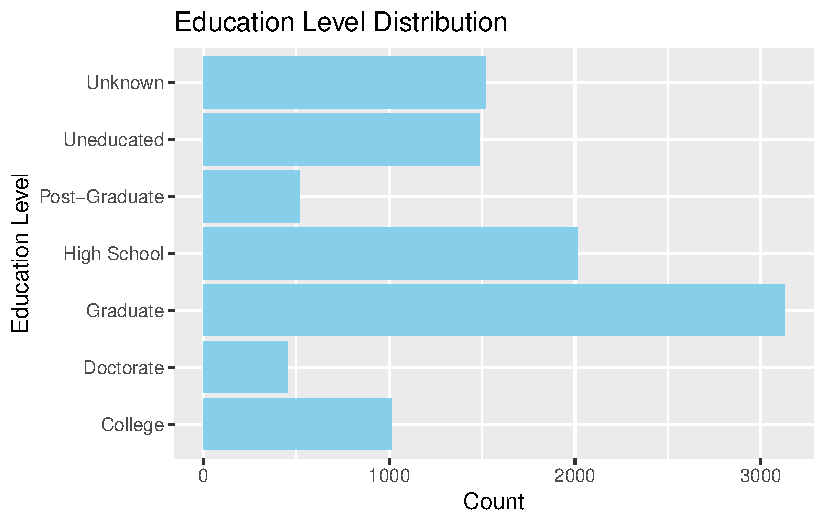
\includegraphics{Tackling-Attrition-at-Tifosi-Bank_files/figure-pdf/unnamed-chunk-7-1.pdf}

\begin{Shaded}
\begin{Highlighting}[]
\FunctionTok{library}\NormalTok{(dplyr)}
\FunctionTok{library}\NormalTok{(forcats)}

\CommentTok{\# 先計算每個 level 的比例}
\NormalTok{level\_summary }\OtherTok{\textless{}{-}}\NormalTok{ data }\SpecialCharTok{\%\textgreater{}\%}
  \FunctionTok{count}\NormalTok{(education\_level) }\SpecialCharTok{\%\textgreater{}\%}
  \FunctionTok{mutate}\NormalTok{(}\AttributeTok{prop =}\NormalTok{ n }\SpecialCharTok{/} \FunctionTok{sum}\NormalTok{(n))  }\CommentTok{\#  算出每個類別佔全部樣本的比例 }

\CommentTok{\# 決定閾值(比如5\%以下算 rare)}
\NormalTok{threshold }\OtherTok{\textless{}{-}} \FloatTok{0.05}

\CommentTok{\# 標記 rare / common}
\NormalTok{data }\OtherTok{\textless{}{-}}\NormalTok{ data }\SpecialCharTok{\%\textgreater{}\%}
  \FunctionTok{left\_join}\NormalTok{(level\_summary, }\AttributeTok{by =} \StringTok{"education\_level"}\NormalTok{) }\SpecialCharTok{\%\textgreater{}\%}
  \FunctionTok{mutate}\NormalTok{(}
    \AttributeTok{small\_level =} \FunctionTok{if\_else}\NormalTok{(prop }\SpecialCharTok{\textless{}}\NormalTok{ threshold, }\StringTok{"Rare"}\NormalTok{, }\StringTok{"Common"}\NormalTok{)}
\NormalTok{  ) }\CommentTok{\#把 level\_summary 的 n 和 prop 合併到 data,以 education\_level 為鍵}

\NormalTok{data }\SpecialCharTok{\%\textgreater{}\%}
  \FunctionTok{ggplot}\NormalTok{(}\FunctionTok{aes}\NormalTok{(}\AttributeTok{x =} \FunctionTok{fct\_infreq}\NormalTok{(education\_level), }\AttributeTok{fill =}\NormalTok{ small\_level)) }\SpecialCharTok{+}
  \FunctionTok{geom\_bar}\NormalTok{() }\SpecialCharTok{+}
  \FunctionTok{coord\_flip}\NormalTok{() }\SpecialCharTok{+}
  \FunctionTok{labs}\NormalTok{(}\AttributeTok{title =} \StringTok{"Education Level Distribution Highlighting Rare Levels"}\NormalTok{,}
       \AttributeTok{x =} \StringTok{"Education Level"}\NormalTok{,}
       \AttributeTok{y =} \StringTok{"Count"}\NormalTok{) }\SpecialCharTok{+}
  \FunctionTok{scale\_fill\_manual}\NormalTok{(}\AttributeTok{values =} \FunctionTok{c}\NormalTok{(}\StringTok{"Common"} \OtherTok{=} \StringTok{"skyblue"}\NormalTok{, }\StringTok{"Rare"} \OtherTok{=} \StringTok{"red"}\NormalTok{)) }\SpecialCharTok{+}
  \FunctionTok{theme\_minimal}\NormalTok{()}
\end{Highlighting}
\end{Shaded}

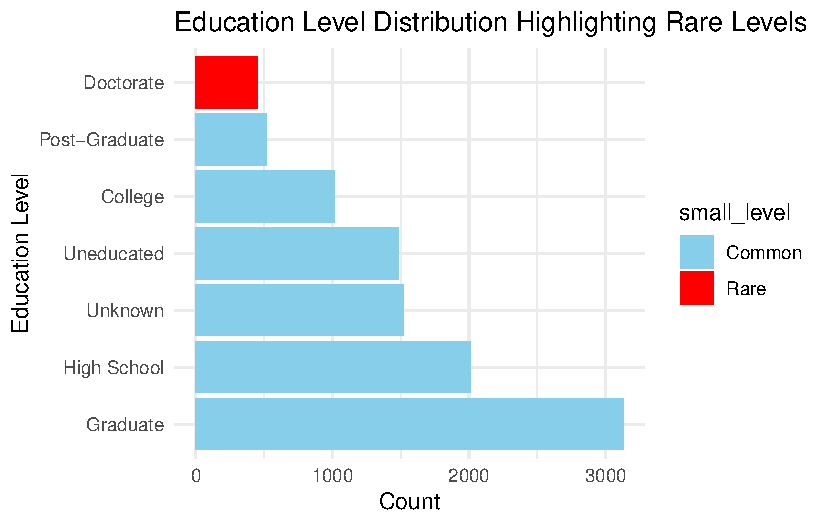
\includegraphics{Tackling-Attrition-at-Tifosi-Bank_files/figure-pdf/unnamed-chunk-7-2.pdf}

\begin{Shaded}
\begin{Highlighting}[]
\FunctionTok{library}\NormalTok{(ggplot2)}
\FunctionTok{library}\NormalTok{(dplyr)}

\CommentTok{\# 指定要畫的變數}
\NormalTok{factor\_vars }\OtherTok{\textless{}{-}} \FunctionTok{c}\NormalTok{(}\StringTok{"attrition\_flag"}\NormalTok{, }\StringTok{"gender"}\NormalTok{, }\StringTok{"education\_level"}\NormalTok{, }
                 \StringTok{"marital\_status"}\NormalTok{, }\StringTok{"income\_category"}\NormalTok{, }\StringTok{"card\_category"}\NormalTok{)}

\CommentTok{\# 用 for loop 自動畫每個}
\ControlFlowTok{for}\NormalTok{ (var }\ControlFlowTok{in}\NormalTok{ factor\_vars) \{}
  
\NormalTok{  data }\SpecialCharTok{\%\textgreater{}\%}
    \FunctionTok{ggplot}\NormalTok{(}\FunctionTok{aes\_string}\NormalTok{(}\AttributeTok{x =}\NormalTok{ var)) }\SpecialCharTok{+}
    \FunctionTok{geom\_bar}\NormalTok{(}\AttributeTok{fill =} \StringTok{"skyblue"}\NormalTok{) }\SpecialCharTok{+}
    \FunctionTok{coord\_flip}\NormalTok{() }\SpecialCharTok{+}
    \FunctionTok{labs}\NormalTok{(}
      \AttributeTok{title =} \FunctionTok{paste}\NormalTok{(}\StringTok{"Distribution of"}\NormalTok{, var),}
      \AttributeTok{x =}\NormalTok{ var,}
      \AttributeTok{y =} \StringTok{"Count"}
\NormalTok{    ) }\SpecialCharTok{+}
    \FunctionTok{theme\_minimal}\NormalTok{() }\OtherTok{{-}\textgreater{}}\NormalTok{ p}
  
  \FunctionTok{print}\NormalTok{(p)}
\NormalTok{\}}
\end{Highlighting}
\end{Shaded}

\begin{verbatim}
Warning: `aes_string()` was deprecated in ggplot2 3.0.0.
i Please use tidy evaluation idioms with `aes()`.
i See also `vignette("ggplot2-in-packages")` for more information.
\end{verbatim}

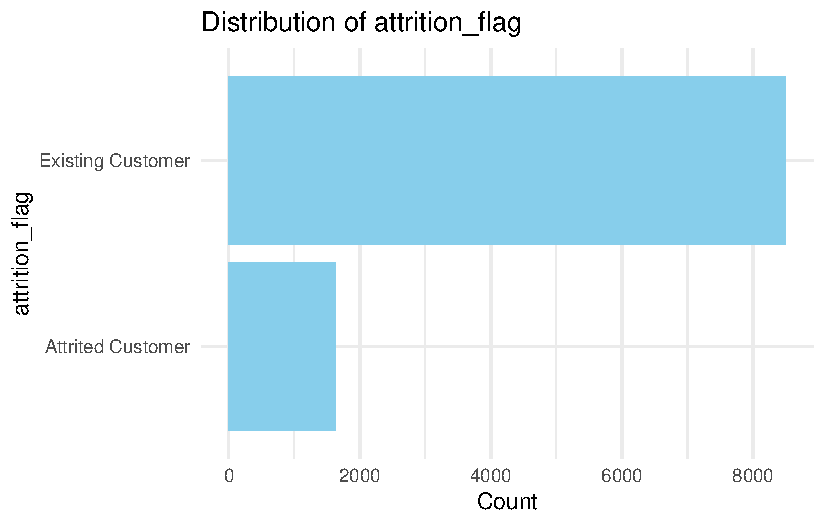
\includegraphics{Tackling-Attrition-at-Tifosi-Bank_files/figure-pdf/unnamed-chunk-8-1.pdf}

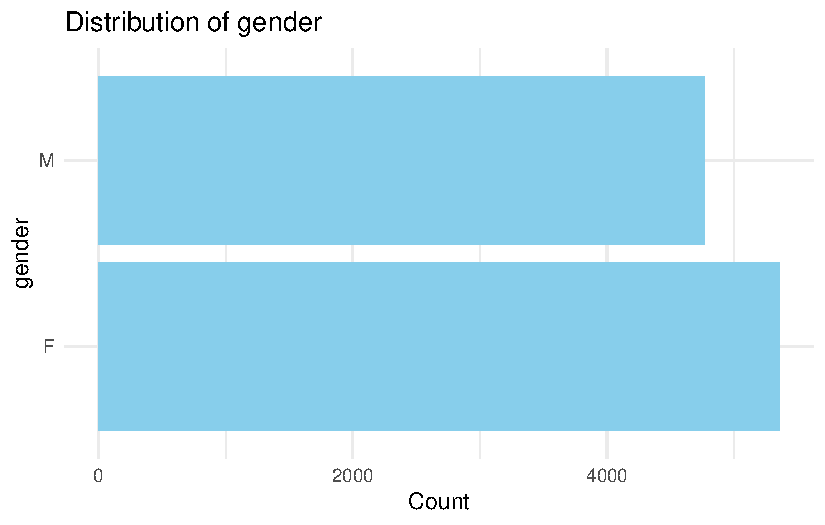
\includegraphics{Tackling-Attrition-at-Tifosi-Bank_files/figure-pdf/unnamed-chunk-8-2.pdf}

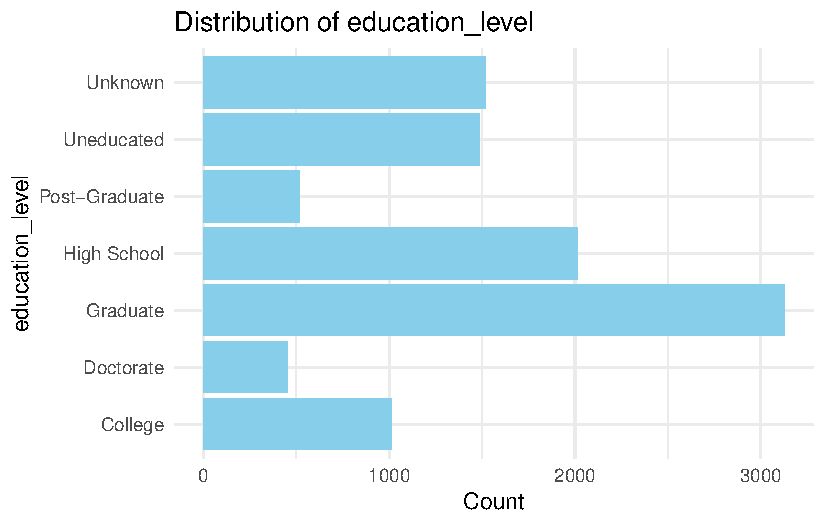
\includegraphics{Tackling-Attrition-at-Tifosi-Bank_files/figure-pdf/unnamed-chunk-8-3.pdf}

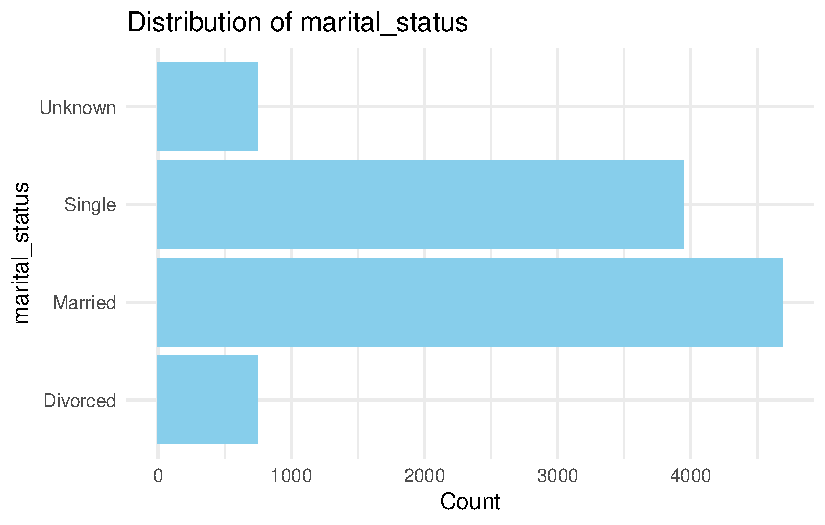
\includegraphics{Tackling-Attrition-at-Tifosi-Bank_files/figure-pdf/unnamed-chunk-8-4.pdf}

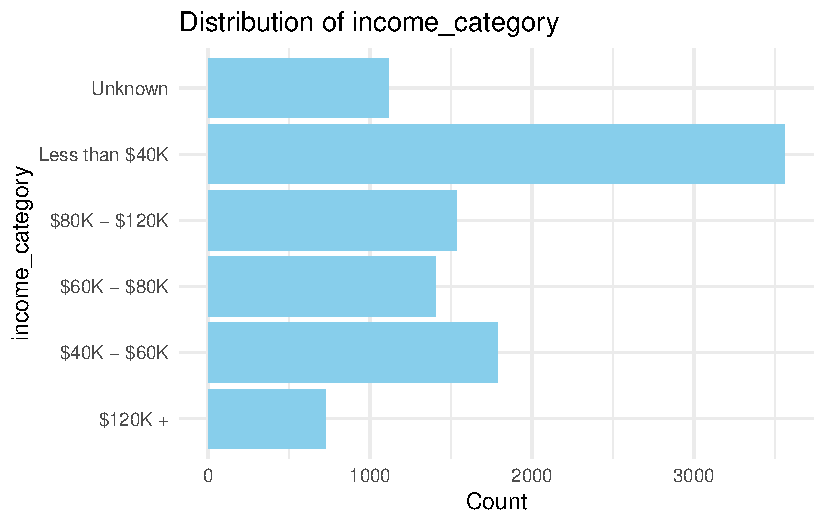
\includegraphics{Tackling-Attrition-at-Tifosi-Bank_files/figure-pdf/unnamed-chunk-8-5.pdf}

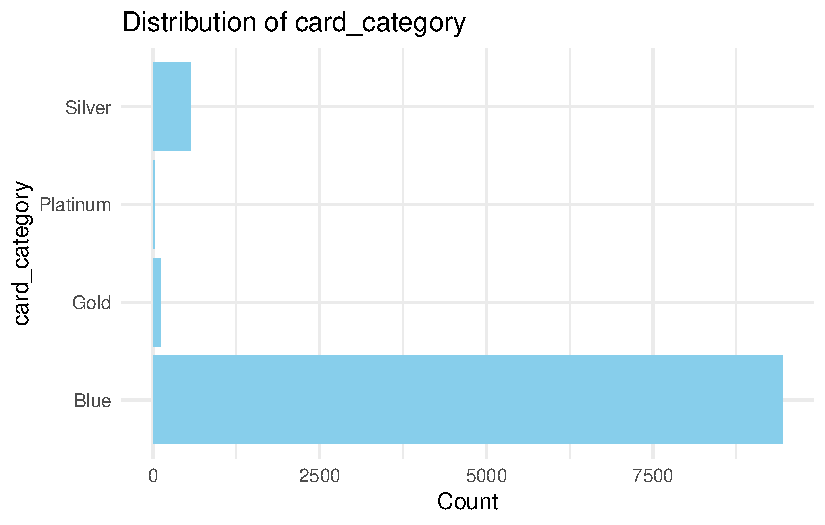
\includegraphics{Tackling-Attrition-at-Tifosi-Bank_files/figure-pdf/unnamed-chunk-8-6.pdf}

\paragraph{response variable}\label{response-variable}

\begin{Shaded}
\begin{Highlighting}[]
\FunctionTok{library}\NormalTok{(ggplot2)}

\FunctionTok{ggplot}\NormalTok{(data, }\FunctionTok{aes}\NormalTok{(}\AttributeTok{x =}\NormalTok{ attrition\_flag)) }\SpecialCharTok{+}
  \FunctionTok{geom\_bar}\NormalTok{(}\AttributeTok{fill =} \StringTok{"skyblue"}\NormalTok{) }\SpecialCharTok{+}
  \FunctionTok{geom\_text}\NormalTok{(}\AttributeTok{stat =} \StringTok{"count"}\NormalTok{, }\FunctionTok{aes}\NormalTok{(}\AttributeTok{label =} \FunctionTok{after\_stat}\NormalTok{(count)), }\AttributeTok{hjust =} \FloatTok{0.2}\NormalTok{) }\SpecialCharTok{+} 
  \FunctionTok{coord\_flip}\NormalTok{() }\SpecialCharTok{+}  \CommentTok{\#after\_stat(count)}
  \FunctionTok{labs}\NormalTok{(}\AttributeTok{title =} \StringTok{"Attrition Flag Distribution"}\NormalTok{,}
       \AttributeTok{x =} \StringTok{"Customer Status"}\NormalTok{,}
       \AttributeTok{y =} \StringTok{"Count"}\NormalTok{) }\SpecialCharTok{+}
  \FunctionTok{theme\_minimal}\NormalTok{()}
\end{Highlighting}
\end{Shaded}

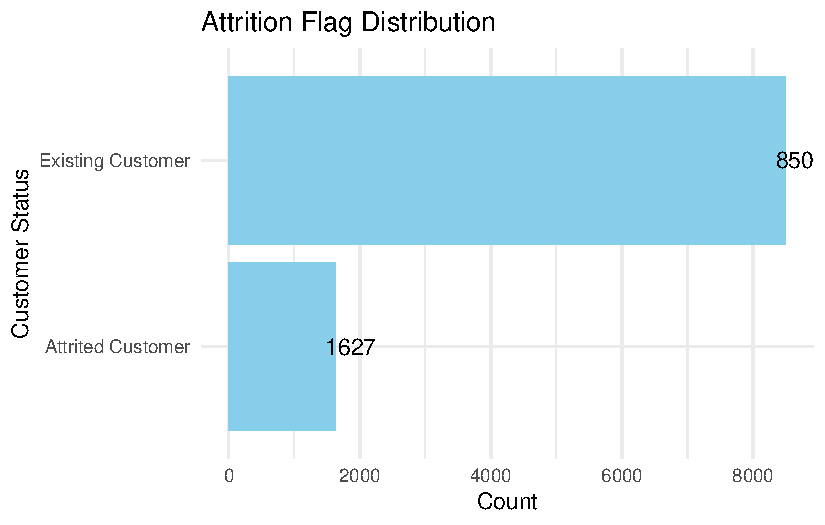
\includegraphics{Tackling-Attrition-at-Tifosi-Bank_files/figure-pdf/unnamed-chunk-9-1.pdf}

\paragraph{relationships among the numerical
variables}\label{relationships-among-the-numerical-variables}

\begin{Shaded}
\begin{Highlighting}[]
\FunctionTok{library}\NormalTok{(GGally)}
\end{Highlighting}
\end{Shaded}

\begin{verbatim}
Warning: package 'GGally' was built under R version 4.3.2
\end{verbatim}

\begin{Shaded}
\begin{Highlighting}[]
\NormalTok{data }\SpecialCharTok{\%\textgreater{}\%} 
   \FunctionTok{select}\NormalTok{(}\FunctionTok{where}\NormalTok{(is.numeric)) }\SpecialCharTok{\%\textgreater{}\%} 
\NormalTok{  GGally}\SpecialCharTok{::}\FunctionTok{ggpairs}\NormalTok{(}\AttributeTok{upper =} \FunctionTok{list}\NormalTok{(}\AttributeTok{continuous =} \FunctionTok{wrap}\NormalTok{(}\StringTok{"cor"}\NormalTok{, }\AttributeTok{size =} \DecValTok{2}\NormalTok{)))}
\end{Highlighting}
\end{Shaded}

\includegraphics{Tackling-Attrition-at-Tifosi-Bank_files/figure-pdf/unnamed-chunk-10-1.pdf}

\begin{Shaded}
\begin{Highlighting}[]
\CommentTok{\#Pearson correlation 測試線性強度}
\end{Highlighting}
\end{Shaded}

\begin{Shaded}
\begin{Highlighting}[]
\FunctionTok{library}\NormalTok{(dplyr)}
\FunctionTok{library}\NormalTok{(tidyr)}

\CommentTok{\# 設定你的數值變數資料(只選 numeric)}
\NormalTok{numeric\_data }\OtherTok{\textless{}{-}}\NormalTok{ data }\SpecialCharTok{\%\textgreater{}\%} \FunctionTok{select}\NormalTok{(}\FunctionTok{where}\NormalTok{(is.numeric))}

\CommentTok{\# 計算 correlation matrix}
\NormalTok{cor\_matrix }\OtherTok{\textless{}{-}} \FunctionTok{cor}\NormalTok{(numeric\_data, }\AttributeTok{use =} \StringTok{"complete.obs"}\NormalTok{)}

\CommentTok{\# 把 correlation matrix 轉成長格式}
\NormalTok{cor\_df }\OtherTok{\textless{}{-}} \FunctionTok{as.data.frame}\NormalTok{(}\FunctionTok{as.table}\NormalTok{(cor\_matrix))}

\CommentTok{\# 避免重複(只保留上三角)}
\NormalTok{cor\_df }\OtherTok{\textless{}{-}}\NormalTok{ cor\_df }\SpecialCharTok{\%\textgreater{}\%}
  \FunctionTok{filter}\NormalTok{(}\FunctionTok{as.character}\NormalTok{(Var1) }\SpecialCharTok{\textless{}} \FunctionTok{as.character}\NormalTok{(Var2)) }

\CommentTok{\# 篩選出高相關變數對}
\NormalTok{high\_cor }\OtherTok{\textless{}{-}}\NormalTok{ cor\_df }\SpecialCharTok{\%\textgreater{}\%}
  \FunctionTok{filter}\NormalTok{(}\FunctionTok{abs}\NormalTok{(Freq) }\SpecialCharTok{\textgreater{}} \FloatTok{0.7}\NormalTok{) }\SpecialCharTok{\%\textgreater{}\%}
  \FunctionTok{arrange}\NormalTok{(}\FunctionTok{desc}\NormalTok{(}\FunctionTok{abs}\NormalTok{(Freq)))}

\CommentTok{\# 顯示結果}
\NormalTok{high\_cor}
\end{Highlighting}
\end{Shaded}

\begin{verbatim}
             Var1           Var2      Freq
1               n           prop 1.0000000
2 avg_open_to_buy   credit_limit 0.9959805
3 total_trans_amt total_trans_ct 0.8071920
4    customer_age months_on_book 0.7889124
\end{verbatim}

\begin{Shaded}
\begin{Highlighting}[]
\FunctionTok{library}\NormalTok{(ggplot2)}

\NormalTok{data }\SpecialCharTok{\%\textgreater{}\%}
  \FunctionTok{ggplot}\NormalTok{(}\FunctionTok{aes}\NormalTok{(}\AttributeTok{x =}\NormalTok{ education\_level, }\AttributeTok{fill =}\NormalTok{ attrition\_flag)) }\SpecialCharTok{+}
  \FunctionTok{geom\_bar}\NormalTok{(}\AttributeTok{position =} \StringTok{"fill"}\NormalTok{) }\SpecialCharTok{+}
  \FunctionTok{coord\_flip}\NormalTok{() }\SpecialCharTok{+}
  \FunctionTok{labs}\NormalTok{(}
    \AttributeTok{x =} \StringTok{"Education Level"}\NormalTok{,}
    \AttributeTok{y =} \StringTok{"Proportion"}\NormalTok{,}
    \AttributeTok{title =} \StringTok{"Proportion of Attrition by Education Level"}
\NormalTok{  ) }\SpecialCharTok{+}
  \FunctionTok{theme\_minimal}\NormalTok{() }\SpecialCharTok{+}
  \FunctionTok{scale\_fill\_manual}\NormalTok{(}\AttributeTok{values =} \FunctionTok{c}\NormalTok{(}\StringTok{"skyblue"}\NormalTok{, }\StringTok{"red"}\NormalTok{)) }\SpecialCharTok{+}
  \FunctionTok{theme}\NormalTok{(}\AttributeTok{axis.text.x =} \FunctionTok{element\_text}\NormalTok{(}\AttributeTok{angle =} \DecValTok{30}\NormalTok{, }\AttributeTok{hjust =} \DecValTok{1}\NormalTok{))}
\end{Highlighting}
\end{Shaded}

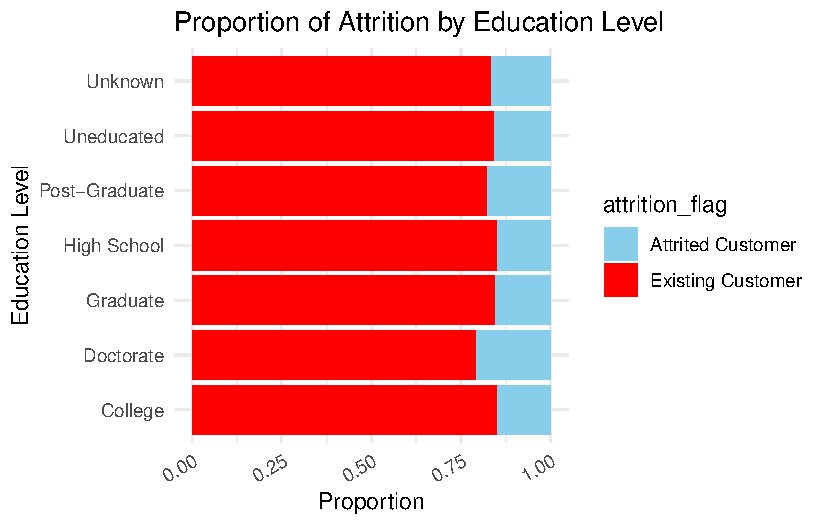
\includegraphics{Tackling-Attrition-at-Tifosi-Bank_files/figure-pdf/unnamed-chunk-12-1.pdf}

\begin{Shaded}
\begin{Highlighting}[]
\FunctionTok{library}\NormalTok{(ggplot2)}
\FunctionTok{library}\NormalTok{(dplyr)}
\FunctionTok{library}\NormalTok{(forcats)}

\CommentTok{\# 先列出你要分析的 categorical predictors}
\NormalTok{factor\_vars }\OtherTok{\textless{}{-}} \FunctionTok{c}\NormalTok{(}\StringTok{"gender"}\NormalTok{, }\StringTok{"education\_level"}\NormalTok{, }\StringTok{"marital\_status"}\NormalTok{, }\StringTok{"income\_category"}\NormalTok{, }\StringTok{"card\_category"}\NormalTok{)}

\CommentTok{\# 重新整理資料:轉成長格式(方便畫 facet\_wrap)}
\NormalTok{data\_long }\OtherTok{\textless{}{-}}\NormalTok{ data }\SpecialCharTok{\%\textgreater{}\%}
  \FunctionTok{select}\NormalTok{(}\FunctionTok{all\_of}\NormalTok{(factor\_vars), attrition\_flag) }\SpecialCharTok{\%\textgreater{}\%}
  \FunctionTok{pivot\_longer}\NormalTok{(}\AttributeTok{cols =} \SpecialCharTok{{-}}\NormalTok{attrition\_flag, }\AttributeTok{names\_to =} \StringTok{"predictor"}\NormalTok{, }\AttributeTok{values\_to =} \StringTok{"level"}\NormalTok{)}

\CommentTok{\# 畫圖}
\FunctionTok{ggplot}\NormalTok{(data\_long, }\FunctionTok{aes}\NormalTok{(}\AttributeTok{x =}\NormalTok{ level, }\AttributeTok{fill =}\NormalTok{ attrition\_flag)) }\SpecialCharTok{+}
  \FunctionTok{geom\_bar}\NormalTok{(}\AttributeTok{position =} \StringTok{"fill"}\NormalTok{) }\SpecialCharTok{+}
  \FunctionTok{facet\_wrap}\NormalTok{(}\SpecialCharTok{\textasciitilde{}}\NormalTok{ predictor, }\AttributeTok{scales =} \StringTok{"free\_x"}\NormalTok{) }\SpecialCharTok{+}
  \FunctionTok{coord\_flip}\NormalTok{() }\SpecialCharTok{+}
  \FunctionTok{labs}\NormalTok{(}
    \AttributeTok{title =} \StringTok{"Proportion of Attrition by Categorical Predictors"}\NormalTok{,}
    \AttributeTok{x =} \StringTok{"Levels"}\NormalTok{,}
    \AttributeTok{y =} \StringTok{"Proportion"}
\NormalTok{  ) }\SpecialCharTok{+}
  \FunctionTok{scale\_fill\_manual}\NormalTok{(}\AttributeTok{values =} \FunctionTok{c}\NormalTok{(}\StringTok{"skyblue"}\NormalTok{, }\StringTok{"red"}\NormalTok{)) }\SpecialCharTok{+}
  \FunctionTok{theme\_minimal}\NormalTok{() }\SpecialCharTok{+}
  \FunctionTok{theme}\NormalTok{(}\AttributeTok{axis.text.x =} \FunctionTok{element\_text}\NormalTok{(}\AttributeTok{angle =} \DecValTok{30}\NormalTok{, }\AttributeTok{hjust =} \DecValTok{1}\NormalTok{))}
\end{Highlighting}
\end{Shaded}

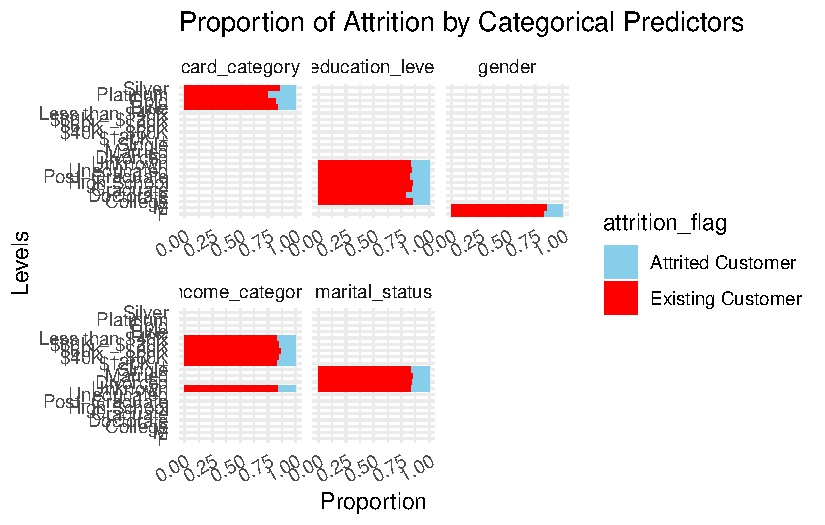
\includegraphics{Tackling-Attrition-at-Tifosi-Bank_files/figure-pdf/unnamed-chunk-13-1.pdf}




\end{document}
